\subsection{$\beta$ validation on binary Mnist digit classification}

\subsubsection{Motivation}

When we explore the derivative \(\frac{dh}{dw_i}\), the role of \(\beta\) becomes paramount:

\textbf{Small Values of \(\beta\):}
As \(\beta \to 0\), \(\frac{dh}{dw_i}\) essentially becomes:
\[ \frac{dh}{dw_i} \approx \int k_i(t) \, dt \]

With a small \(\beta\), the model averages the responses across time. This means it doesn't pay much attention to the timing of each spike. This is similar to a perceptron that sums up inputs scalar.

\textbf{Large Values of \(\beta\):}
For high values of \(\beta\), \(\frac{dh}{dw_i}\) converges to:
\[ \frac{dh}{dw_i} \approx k_i(t_{\text{max}}) \]
where \(t_{\text{max}}\) is the time instant that maximizes \(v(t)\).

For a large \(\beta\), the neuron mainly reacts when \(v(t)\) is at its peak. This is similar to how the max-time tempotron focuses on the exact moment the input reaches a peak.

Essentially, the value of \(\beta\) is crucial for the tempotron's interpretation of time. A smaller \(\beta\) causes the neuron to blend inputs over time, resembling the behavior of a perceptron. On the other hand, a larger \(\beta\) emphasizes the most significant moments of input, akin to the max-time tempotron, which highlights peak input times.

\subsubsection{Experimental Framework}

The main aim of this experiment is to assess how the convolution-based Tempotron model performs on Mnist odd and even digits, particularly when adjusting the values of $\beta$.

\subsubsection{Input Data}

The Mnist Digits dataset was utilized, separating it based on odd and even digits, represented by a binary label. Each $28 \times 28$ image was transformed into a 784-length vector, normalized to lie within the range [0, 1]. The data was then encoded using the rate encoding method detailed in section \ref{ssec:rate-encoding-method}.


\subsubsection{Model Architecture}

The Convolution-based Tempotron model's design and operational mechanics are detailed in section \ref{sssec:training-conv-cost} on \textbf{Methods}.


\subsubsection{Procedure}

For each selected $\beta$ value, multiple experimental trials were executed, each undergoing a preset number of learning iterations (or until training convergence), processing data in specified batch sizes.

\subsubsection{Parameter Descriptions}

\begin{enumerate}
    \item \textbf{Duration \( T \): 500 ms} \\
    Represents the length of time for which the model will simulate the neural dynamics for each given input pattern.
    
    \item \textbf{Time step \( dt \): 1 ms} \\
    The sampling time at which we "measure" the experiment.
    
    \item \textbf{Potential Scaling Factor \( V_0 \): 2.12} 
    
    \item \textbf{Firing threshold \( V_{th} \): 1} \\
    The potential level at which a neuron emits a spike. When the neuron's membrane potential exceeds $V_{th}$, it "fires" or produces an output spike.
    
    \item \textbf{Time constant \( \tau \): 10 ms} \\
    Determines the rate at which a neuron's membrane potential decays back towards its resting potential after perturbation.

    \item \textbf{Max rate \( R \): 20 Hz} \\
    Determines the maximum rate at which a neuron fires.
    
    \item \textbf{Output layer size: 1 neuron} \\
    Indicates the number of neurons in the model's final layer, which produces the final decision or classification.
    
    \item \textbf{Maximum iterations: 750} 

    \item \textbf{Batch size: 64} \\
    Dictates how many input patterns are processed simultaneously before updating the model's internal parameters. 

\end{enumerate}

\subsubsection{Results}

\begin{figure}[H]
    \centering
    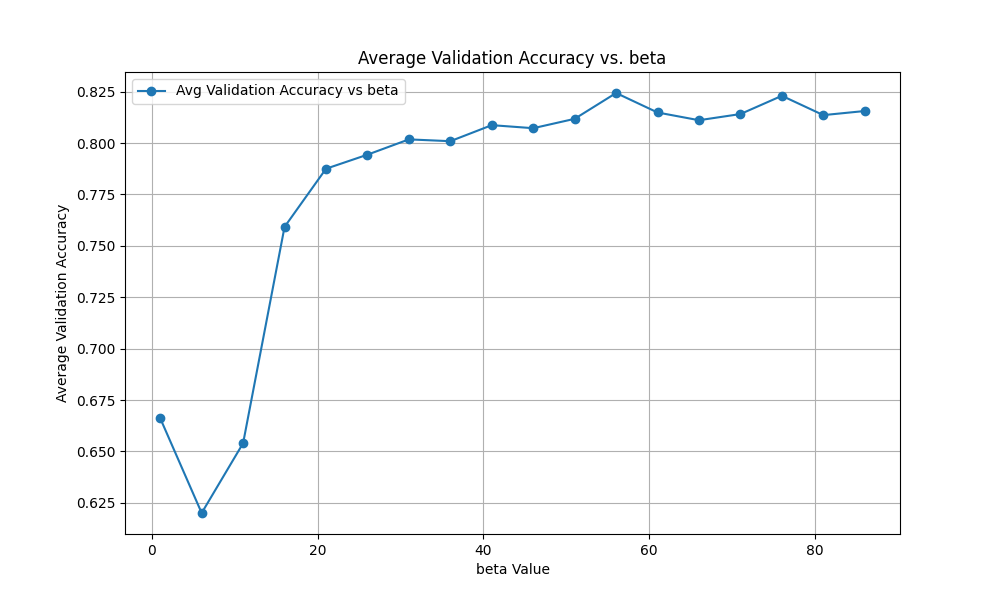
\includegraphics[width=0.8\linewidth]{results/graphs/beta-validation.png}
    \caption{Average test accuracy as a function of $\beta$}
    \label{fig:beta-validation}
\end{figure}


\subsubsection{Observation}

